\chapter{Cognitive theories}

\label{ch:theory}

This chapter aims to explain the effectivity and inner workings of both concept mapping and flashcard systems by elaborating on the physiology of the relevant parts of the brain, and the relevant cognitive theories. It is important however that these theories mainly focus on a certain type of learning only. According to \citeA{squire}, there are multiple varieties of memory, which can mainly be categorised into declarative and nondeclarative knowledge, sometimes also referred to as respectively explicit and implicit knowledge \citeA{cognitivepsychology}. Declarative knowledge also refers to memories that can be explicitly recalled, entailing facts such as definitions, paired associations etc., but also the events where these facts were acquired. Nondeclarative memory involves every memory which can be demonstrated in action, but not in conscious recall per se. Subcategories of these memories are procedural skills, priming, conditioning, and nonassociative memories. Because of the nature of this study, the cognitive theories discussed below are mainly focused on declarative knowledge, although most theories also are relevant to nondeclarative memory in some degree.

Furthermore, \citeA{instructionaldesign} describes declarative knowledge as one of Gagné's types of learning outcomes, and relates declarative knowledge to Bloom's levels of recall and understanding, meaning that declarative knowledge does not only encompass rote memorisation of facts, but also understanding the meaning behind this fact. This is also in line with the essay written by \citeA{glaserfield} on radical constructivism, in which it is stated that whatever it is that students are to place into memory they should also understand. Another category of learning outcomes applicable to this context is that of intellectual skills, mainly that of concepts. These, according to \citeA{instructionaldesign}, help the learners simplify the world and can make them into more efficient thinkers. From a cognitive perspective however, there is not a great difference in dealing with declarative knowledge or concepts, because both relate to explicitly recallable memories and thereby can both be considered as being explicit \cite{squire}.

\section{Storage and retrieval}

\begin{figure}
    \centering
    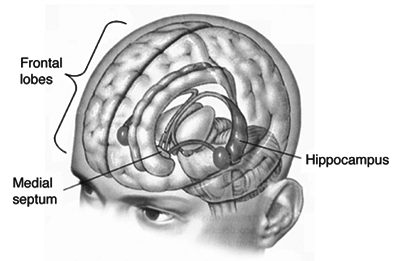
\includegraphics[width=0.5\textwidth]{img/brainareas.png}
    \caption{The brain areas mainly involved in storing and retrieving declarative knowledge \protect\cite{amnesia}}
    \label{fig:brainareas}
\end{figure}

Although the whole brain is involved in storing memories, the most prominent areas facilitating the process of memorising are the frontal lobes, medial septum and the hippocampus \cite{cognitivepsychology} (see figure~\ref{fig:brainareas}). The prefrontal regions are responsible for the creation and retrieval of memories, whereas the hippocampal and surrounding areas allow permanent storage of these memories. Because of this dynamic, \citeA{modalmemory} conceived a modal theory of memory, displayed in figure~\ref{fig:modalmemory}. In this model, information is perceived as sensory input, and is then shortly stored in the sensory memory. If the perceiver has paid enough attention to the input, it is then transfered (or encoded) into short-term memory. When the input is strong enough, that is, rehearsed often enough within short term memory, it can be more permanently stored in long-term memory. If not, the input fades away from memory and is forgotten. When a memory exists in long-term memory, it has to be retrieved into short-term memory in order to be remembered and used.

This model was heavily influenced by developments in electrical engineering and computer sciences, and can be thought of as functioning like a complex computer, where data is written on a hard drive (the long-term memory), and can be used by first retrieving it into working memory (or short-term memory) and later be transferred to the hard drive again (although within a computer the separation is much more clear, whereas short- and long-term memory might overlap more). However, the way the brain works is different from a computer in the sense that a brain has to put effort into memorising data, and that a brain forgets data over time. Therefore, instead of merely inputting the data, learning requires a more rigid approach.

\begin{figure}
    \centering
    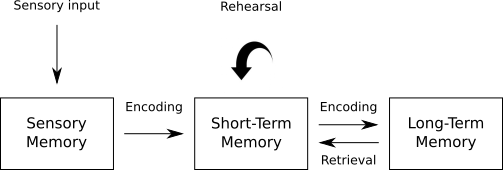
\includegraphics[width=0.5\textwidth]{img/modalmemory.png}
    \caption{The modal model of memory proposed by \protect\citeA{modalmemory}}
    \label{fig:modalmemory}
\end{figure}

\citeA{karpicke4} describes two seperate learning practices based on the modal model of memory, namely encoding and retrieval practices, where encoding practices are focused on meaningful encoding or construction of knowledge, and retrieval practiced are more focused on the reconstruction and rehearsal of knowledge. He states that both practices are essential to enhancing learning. Flashcards are a famous retrieval practice, which emphasise drilling the same pairs by association over and over again, whereas concept maps are known to be an encoding practice where the student has to connect diverse concepts within one topic by meaningful relations.

The following sections will elaborate on cognitive effects with regard to both encoding and retrieval practices, and relating them with their relevance to the effectiveness of concept mapping and flashcard systems respectively.

\section{Cognitive effects with regard to encoding practices}

The first step of memorisation is always encoding, because (logically speaking) a stimulus first has to be processed and encoded in either short-term or long-term memory in order to be retrieved or used later on. After all, one cannot retrieve a memory which is not already there. It therefore is important to first acknowledge by which means knowledge is encoded, and in what kind of structure it is then stored.

\subsection{Early metaphors for the brain}

For centuries, a lot of metaphors describing memory depicted the brain as a room in which a person could store physical things, for example as a library filled with books or a storehouse with items \cite{roediger}. This metaphor seems intuitive and is easy to understand, hence it is still prevalent today. There even exists a widely-used memorisation technique called the \emph{loci method}, which lets students are asked to imagine a house where they have to store memories as physical objects in the room. They can then later retrieve the memories by walking through the house along the objects they have stored the memories in \cite{cognitivepsychology}.


Yet, this model still has certain flaws. Firstly, with regards to retrieval practices, it depicts memories as static objects which only have to be stored to be remembered forever, misleading students, teachers and scientists into focusing more on encoding practices than on retrieval practices \cite{karpicke4}. Furthermore, memories are imagined as separate objects, which does not correspond with how memories are encoded in the brain. As a matter of fact, already in the 19th century, Cajal discovered that memories were patterns of electrical neural activity leading to synaptic changes \cite{longtermpotentiation}. This enabled another spatial metaphor, namely that of a switchboard, where the synapses were represented by electrical wires \cite{roediger}. Later on, when the field of computer science begun to emerge, this metaphor transformed to that of a computer, enabling the conception of the modal model of memory. This is already a more useful metaphor than the physical space metaphor, since it is more biologically accurate, and it emphasises the need of communication between certain nodes (encoding and retrieval between the different memory systems).

However, the metaphor of a computer still has its flaws. A computer stores information on certain independent addresses in the form of binary data, and thereby implies that one can store data for later use without any need for comprehension of the data, and that the data can be formatted in any way the user would like to. Yet, the brain is differently structured, which has consequences for succesfull encoding.

\subsection{The brain as an associative network}

Unlike a computer, the brain is not organised into bits with physical addresses, but rather structured as an associative network. This entails the data being stored and retrieved by means of associated peers. In the brain, the neurons function as the nodes, and the synapses function as the edges. When information is encoded, new neurons are marked, and these are connected to other relevant, already marked neurons in the network. When something then has to be retrieved from memory, neurons signal relevant neighbouring neurons in order to activate the relevant parts of the brain. More generally speaking, when stimulated with a retrieval cue, the brain can then use neural pathways to find a corresponding item in the brain. These networks are sometimes referred to as \emph{semantic networks}, and the implication for retrieval as \emph{spreading activation} \cite{cognitivepsychology}. This effect has also been found on a cognitive level, for example \citeA{kintsch} has found that material is often not literally encoded, but rather as a set of abstract meaning units representing certain associations between concepts.

\subsection{Elaborative processing}

Because information is retrieved in the brain via related nodes and edges in the semantic network, strong neural pathways facilitate the retrieval process. One way of creating these pathways is elaborative processing \cite{karpicke4, cognitivepsychology}, which focuses on meaningful processing of the content. \citeA{craik} conducted an experiment where students were to freely recall from a list of words after the students had to train the words by one of the following techniques: answering questions about structural details (e.g. is it in capital letters); about phonemical details (e.g. the word rhyming on another word); whether the word fits into a certain category; and whether the word fits in a certain sentence. They found that the more meaningful the task was, the higher the retrieval rate was (so the latter techniques were more effective). The same result was found by \citeA{barclay}. Furthermore, research conducted by \citeA{nelson} presented students with paired associates that where either semantic or phonetic (in this case rhymes), and students showed a significantly higher recall of semantic associates. These studies demonstrate the importance of meaningful processing for retention.

\subsection{Implications for concept mapping}

Reflecting on the previously described theory of associated networks, it appears that a semantic network is very similar in structure to concept maps, and thereby the maps provide an accurate representation of the way information is retrieved from the brain. For example, \citeA{canas} states that "the widespread use of concept maps is based on the notion that a concept map is a reflection of the builder's cognitive structure and thus portrays his or her understanding of the domain depicted in the map" (p. 1). \citeA{nesbit} speculate that because of this, more and better retrieval cues are created when learning from or generating a concept map. Furthermore, a concept map displays the relations between certain concepts, and thereby focuses more on the meaning behind the content, rather than just the content itself.

\section{Cognitive effects with regard to retrieval practices}

According to \citeA{karpicke4}, a lot of educational practices have placed an emphasis on finding optimal ways to encode knowledge and experiences, but that retrieval practices have received less attention. Nevertheless, basic research has indicated that retrieval is still important to consider in any analysis of learning. This is mainly due to the fact that information is not stored exactly and indefinitely, but rather that memories are forgotten over time. Two theories have been proposed and debated over explaining why forgetting occurs, namely by interference of other redundant memories and by decay of existing memories.

\subsection{Interference and Decay}

\label{subsec:interferencedecay}

The theory of interference being responsible for forgetting has been demonstrated in an experiment by \citeA{interference}. The participants were asked to memorise sentences in the form \emph{A \textless person\textgreater{} is in the \textless location\textgreater}, where sometimes multiple persons where associated with only one location, and some locations with only one person. They found that if a sentence contained locations or persons with multiple associations this had an impact on the recognition time for that sentence, and even more so if both the location and the person had multiple associations. The explanation for this phenomenon is that since memories are retrieved by means of spreading activation and only limited activation can spread from one source \cite{cognitivepsychology}, the activity has to be divided over different branches in the semantic network, increasing the retrieval difficulty of the correct node. The increase in difficulty is also related to as the \emph{fan effect}.

The effect of decaying memories takes place in the connections between neurons, and therefore it is important to first examine how neurons communicate signals. Figure~\ref{fig:neuron} displays a schematic representation of a neuron in which it can be seen how the soma (cell body) is connected via an axon to the dendritic tree of other cells. The neuron can transmit stimuli by creating an action potential in the nucleus, transmitting this signal through the axon to the terminal button in the connected telodendrion (in the image refered to as the terminal aborization). There, neurotransmitters are released from vesicles, and after they have crossed the synaptic cleft there is a certain chance of being received by postsynaptic receptors. When this is the case, the nucleus of the receiving cell is triggered via the connected dendrite to also create an action potential, and the whole process is repeated \cite{longtermpotentiation}. The strength of a certain connection between neurons is therefore dependent on the action potential generated by a nucleus, the amount of telodendria over which the action potential has to be distributed (hence the aforementioned fan effect), the amount of neurotransmitters in the terminal button, and the amount of postsynaptic receptors in the dendrite of the next neuron.

\begin{figure}
    \centering
    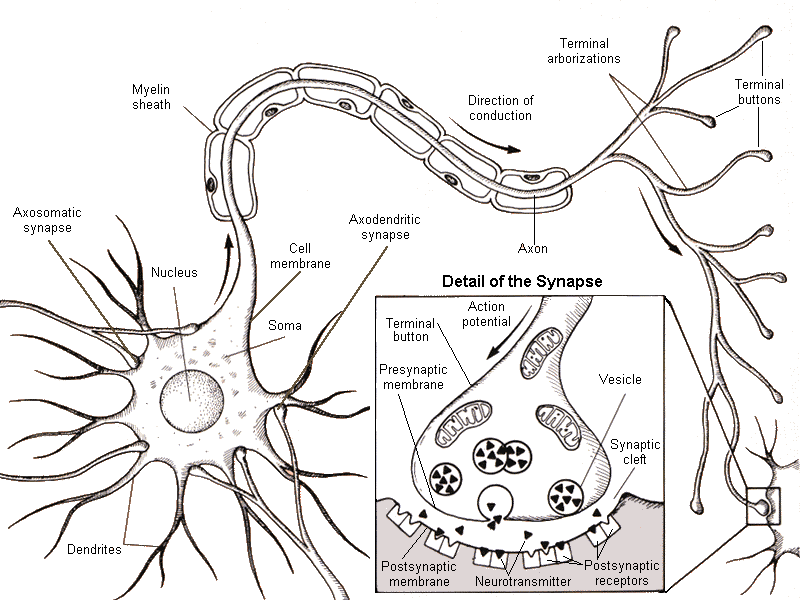
\includegraphics[width=0.8\textwidth]{img/neuron.png}
    \caption{A schematic image of a neuron with a closeup of a synapse \protect\cite{website:neuron}}
    \label{fig:neuron}
\end{figure}

One widely studied effect with regard to the increase and decrease of action potential and strength of memory traces is called long-term potentiation (LTP) \cite{cognitivepsychology, longtermpotentiation, activationbasedmodel, amnesia}. Whenever a neurotransmitter is received by by a receptor, not only is the next nucleus activated to release its action potential, but also more receptors are activated, so that the postsynaptic membrane is able to receive more neurotransmitters at the next activation. Furthermore, another process is activated altering the metabolical profile of the neuron, causing it to create proteins for more stable increased sensitivity towards stimuli. It is also speculated that there might be a retrograde effect, causing presynaptic modifications such as the creation of more neurotransmitters in the presynaptic vessicles \cite{longtermpotentiation}. This all results in an increased sensitivity in the postsynaptic neuron towards action potential in the presynaptic neuron, which then again increases the strength of this particular memory trace. Over time, if a specific neural pathway is not used, the effects of LTP decrease again, causing its strength to decrease and thereby causing decay. This also is a predictor for the \emph{testing effect}, the effect of retrieval strengthening memory more than extra opportunities for further encoding, even when the retrieval is only carried out internally without any outward response \cite{microlearning}.

Although both the effect of interference and decay have been proposed as separate theories and have been debated, they are still mutually inclusive, and \citeA{cognitivepsychology} therefore conludes that forgetting results both from decay and from interference.

\subsection{Power laws of forgetting and learning}

Now that the relevant theories for learning and forgetting have been discussed, it is important to investigate with which rate people learn and forget. Already in 1885, Ebbinghaus discovered the power law of learning, referred to as the inversal exponential nature of forgetting \cite{microlearning, activationbasedmodel}. The implication of this model is that memory not only systematically deteriorates with delay, but also that this loss is negatively accelerated, meaning that the rate of change gets smaller with increasing delay \cite{cognitivepsychology}. \citeA{wickelgren} already proposed the formula $m = \lambda (1 + \beta t)^{-\psi}$, where $m$ is memory strength (the probability of recognition), $t$ is time, $\lambda$ is the state of long-term memory at $t = 0$, $\psi$ is the rate of forgetting, and $\beta$ is the scaling parameter (see figure~\ref{fig:powerlawforgetting}). This formula has also found to be accurate by \citeA{wixted}. Finally, the effect has been directly related to LTP in the rat hippocampus by stimulating neural pathways directly with electrical signals \cite{raymond}.

\begin{figure}
    \centering
    \begin{subfigure}{0.7\textwidth}
        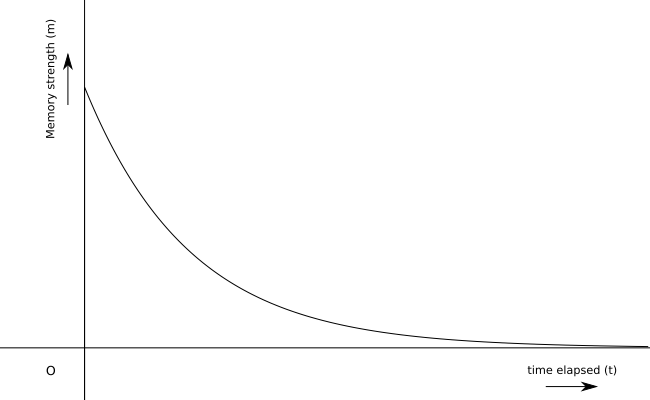
\includegraphics[width=\textwidth]{img/powerlawforgetting}
        \caption{The power law of forgetting, with m as the probability of recognition and t as the time passed since learning}
        \label{fig:powerlawforgetting}
    \end{subfigure}
    \par\bigskip
    \begin{subfigure}{0.7\textwidth}
        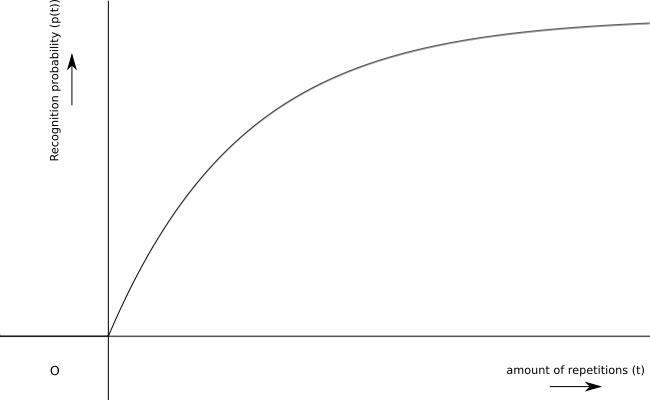
\includegraphics[width=\textwidth]{img/powerlawlearning}
        \caption{The power law of forgetting, with p(t) as the probability of recognition and t as the iterations of learning}
        \label{fig:powerlawlearning}
    \end{subfigure}
    \caption{The power laws of learning and forgetting}
\end{figure}

A similar effect has been found for the effectiveness of repetition: \citeA{powerlaw1} have proposed a power law of learning, stating that a learning curve is inversal exponential (see also \citeA{powerlaw2} and \citeA{powerlaw3}). \citeA{murre} propose $P = p(t) = 1-e^{-\mu_{i}t}$ as a function describing this power law, where $P$ or $p$ is the probability of recognition after $t$ iterations and $\mu$ is the learning rate of student $i$ (see figure~\ref{fig:powerlawlearning}). The power law states that repetition has a positive effect on retrieval probability. This effect however does not increase linearly but inverse exponentially, with an asymptote at a certain amount of repetition. Again, this effect has also been demonstrated in the context of LTP in rat hippocampi \cite{barnes}. The stronger memory trace from a higher repetition rate does not only result in a higher recall probability, but also in a more gradual retention curve, allowing memories to persist longer.

\subsection{Spacing effect}

The spacing effect is a well known effect occuring within paired-associate learning, and demonstrates that repeated items are better remembered when both occurences are separated by other events or items than when they are presented in immediate succession \cite{verkoeijen, logan, siegel, xue, karpicke2}. This effect has been demonstrated with diverse populations \cite{verkoeijen, logan}, under various learning conditions \cite{verkoeijen, logan}, and in both explicit and implicit memory tasks \cite{verkoeijen}. Items in immediate succession are called massed items, and items in separated succession are called spaced items.

One can test the spacing effect either by using pure lists or mixed lists. When using pure lists, one compares the effect of learning a list containing only massed items with a list containing only spaced items, and using mixed lists one measures the effect of learning both massed items and spaced items in one list, comparing their individual retentions. \citeA{verkoeijen} state that the vast majority of studies are conducted using mixed lists and found that spaced items were consistently better recalled than massed items, yet studies using pure lists are relatively rare and have produced contradictory outcomes. They conducted a study providing participants first with an all-massed list, then letting them write down as many words as they could remember, and repeat an identical procedure for an all-spaced list with a 2 minute break inbetween. They conducted this experiment with short-lagged spaced items (with 1-4 items in between) and long-lagged spaced items (with 4-13), and found only a spacing effect in the latter experiment. However, \citeA{wahlheim} adds to this that repetition is only increases when a student detects the repetition of an item, and therefore the lag should not be too long.

Two theories have been presented explaining this phenomenon, namely the contextual variability theory and the study-phase retrieval theory \cite{siegel}. The first theory entails that because context is not static but continuous, and that therefore spaced items are studied in a greater variety of contexts and as such are easier to recall in yet other contexts than massed items due to the so-called encoding-specificity principle \cite{cognitivepsychology}. This principle entails that the probability of recalling an item depends on the similarity of the context during the encoding. The study-phase retrieval theory entails that additional retrieval cues for the repetition of an item are generated by earlier occurences and their associated contexts being associated with the repeated item. These theories are not mutually exclusive \cite{siegel}.

Inspired by the power laws of learning and forgetting, \citeA{karpicke} conducted an experiment to test the effect of constant or varying lags between items on learning. They tested this by conducting a similar experiment to \citeA{verkoeijen}, however in this experiment they only tested pure lists with three different lag intervals to test for an absolute spacing effect. For each lag interval category they tested for an expanding lag condition (where the lag would increase for the repetition of each next item), an equal lag condition (where the lag would remain constant) and a contracting lag condition (where the lag would decrease for the repetition of each next item) in order to test for a relative spacing effect. From their findings they confirmed the effect of absolute spacing, namely that longer gaps between items do have an effect on long-term retention, yet they did not find a relative spacing effect. However, this has not been tested for spacing with longer intervals, such as intervals spanning multiple days or weeks.

\subsection{Implications for the flashcard system}

It can be concluded that the flashcard system derives its effects mainly from the testing effect by having students actively retrieve information instead of simply encoding it, and from the spacing effect by students going through the items interspersally instead of by immediate succession. The key question however is how often a single card has to be repeated. On the one hand, overlearning can occur, where the student repeats an item too often resulting in diminished learning effects because of the power law of learning, and also only on the short term \cite{rohrer}, which is inefficient. On the other hand, if the intervals are too long, students forget the items inbetween intervals, and then the spacing effect does not apply anymore. In order to solve this problem, most modern digital flashcard systems apply a system called \emph{adaptive spaced-repetition learning} (e.g. the Pimsleur system, the Leitner system, Supermemo, and Anki \cite{microlearning}. In this system, exponentially expanding intervals are used, not because of a relative spacing effect which does not exist according to the previously mentioned literature, but rather to increase the average (absolute) spacing with each new repetition. This creates a stronger memory trace every time, but also takes into account the further decreasing risk of forgetting because of the slower declining retention curve (see figure~\ref{fig:spacedrepetition}).

\begin{figure}
    \centering
    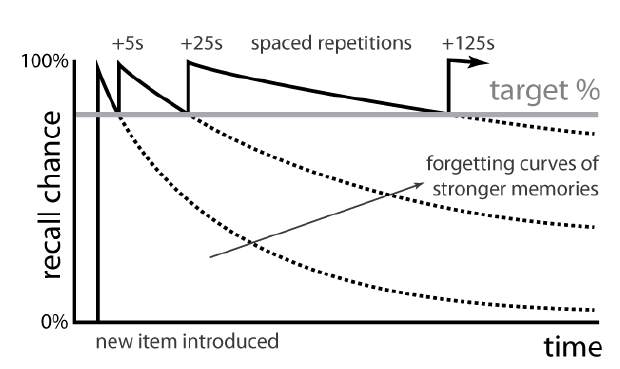
\includegraphics[width=0.5\textwidth]{img/spacedrepetition}
    \caption{Adaptive spaced-repetition learning (taken from \protect\citeA{microlearning})}
    \label{fig:spacedrepetition}
\end{figure}

\section{Conclusion}

Overall, this chapter has discussed several cognitive theories related to the storage and retrieval of explicit (or declarative) knowledge in and from the hippocampus. Related to encoding practices, it has now been established that the brain works as an associative or semantic network, and that meaningful or elaborative processing is important for the later retrieval of memories. This seems to fit with the structure and process of concept mapping, although more research is needed in this area. Furthermore, the theories of interference and decay have been discussed in order to explain forgetting of memories, together with Long-Term Potentiation and its effects on the rate of forgetting and learning. In addition, articles were discussed demonstrating that spaced rehearsal is more effective than massed rehearsal. This has finally led to the conclusion that adaptive spaced-repetition learning is an effective method to expand absolute spacing, which entails that items are repeated with exponentially increasing intervals.
